\documentclass[aspectratio=169]{beamer}

\usetheme{Madrid}
\usecolortheme{seahorse}
\setbeamertemplate{navigation symbols}{}

\usepackage[utf8]{inputenc}
\usepackage[T1]{fontenc}
\usepackage[brazil]{babel}
\usepackage{graphicx}
\usepackage{booktabs}
\usepackage{amsmath}
\usepackage{xcolor}
\usepackage{algorithm}
\usepackage{algpseudocode}
\usepackage{hyperref}

\graphicspath{{../}}

% ── Cores ──────────────────────────────────────────────────────────────────────
\definecolor{ufrjblue}{RGB}{0,83,155}
\definecolor{ufrjgreen}{RGB}{0,150,64}
\setbeamercolor{palette primary}{bg=ufrjblue,fg=white}
\setbeamercolor{palette secondary}{bg=ufrjblue!80,fg=white}
\setbeamercolor{palette tertiary}{bg=ufrjblue!60,fg=white}
\setbeamercolor{structure}{fg=ufrjblue}
\setbeamercolor{block title}{bg=ufrjblue,fg=white}
\setbeamercolor{block body}{bg=ufrjblue!10}

% ── Metadados ──────────────────────────────────────────────────────────────────
\title[Mochila Limitada com GRASP]{Problema da Mochila Limitada\\com Heurística GRASP}
\author{Breno Valente Manhães}
\institute{Otimização Aplicada a Redes \\ UFRJ}
\date{}

% ==============================================================================
\begin{document}
% ==============================================================================

% ── Slide 1: Capa ──────────────────────────────────────────────────────────────
\begin{frame}
  \titlepage
\end{frame}

% ── Slide 2: O Problema ────────────────────────────────────────────────────────
\begin{frame}{O Problema Escolhido: Bounded Knapsack}

  \begin{block}{Definição}
    Dado um conjunto de $n$ itens, cada um com \textbf{valor} $v_i$, \textbf{peso} $w_i$
    e quantidade máxima $q_i$, escolher quantidades inteiras $x_i \in \{0, \ldots, q_i\}$
    que \textbf{maximizem} o valor total sem exceder a capacidade $C$:
    \[
      \max \sum_{i=1}^n v_i x_i \quad \text{s.t.} \quad
      \sum_{i=1}^n w_i x_i \leq C, \quad 0 \leq x_i \leq q_i, \; x_i \in \mathbb{Z}
    \]
  \end{block}

  \vspace{0.5em}
      \textbf{Por que não 0-1?}
      \begin{itemize}
        \item O problema 0-1 força uma escolha binária --- inclui ou não inclui.
        \item A versão \emph{bounded} é mais rica: permite múltiplas unidades por item,
              capturando melhor cenários reais.
      \end{itemize}

\end{frame}

% ── Slide 3: Tentativas Anteriores ─────────────────────────────────────────────
\begin{frame}{Caminho até o GRASP}

  \begin{columns}[T]
    \column{0.48\textwidth}
      \begin{block}{ACO — Ant Colony Optimization}
        \begin{itemize}
          \item Primeira tentativa natural para problemas combinatórios.
          \item Os resultados foram \textbf{decepcionantes}: convergência lenta,
                muito sensível a hiperparâmetros.
          \item Para instâncias grandes ($n > 1000$) o tempo explodiu sem ganhos
                de qualidade expressivos.
        \end{itemize}
      \end{block}
    \column{0.48\textwidth}
      \begin{block}{Algoritmos Genéticos}
        \begin{itemize}
          \item A experiência com ACO gerou ceticismo sobre meta-heurísticas
                baseadas em população para este problema.
          \item Optei por buscar alternativas na literatura.
        \end{itemize}
      \end{block}
  \end{columns}

  \vspace{0.8em}
  \centering
  \large Pesquisando a literatura, encontrei o \textbf{GRASP} ---
  elegante, simples e com boas garantias práticas.

\end{frame}

% ── Slide 4: O GRASP ───────────────────────────────────────────────────────────
\begin{frame}{O Algoritmo GRASP}

  \begin{block}{Referência seminal}
    \textbf{Feo \& Resende (1989)} — \emph{A probabilistic heuristic for a
    computationally difficult set covering problem.}\\
    Operations Research Letters, 8:67–71, 1989.
  \end{block}

  \vspace{0.5em}
  \begin{columns}[T]
    \column{0.5\textwidth}
      \textbf{Estrutura do GRASP}
      \begin{enumerate}
        \item \textbf{Fase de construção} semi-gulosa:\\
              monta uma solução inicial usando aleatoriedade controlada.
        \item \textbf{Fase de busca local}:\\
              refina a solução até um ótimo local.
        \item \textbf{Itera} por um número fixo de vezes,\\
              guardando o melhor resultado.
      \end{enumerate}
    \column{0.5\textwidth}
      \textbf{Por que funciona?}
      \begin{itemize}
        \item Cada iteração parte de um ponto diferente do espaço de busca
              (diversificação).
        \item A busca local garante que cada ponto visitado é um ótimo local
              (intensificação).
        \item Custo por iteração reduzido: $O(n \log n)$ construção +
              $O(n)$ busca local por passo.
      \end{itemize}
  \end{columns}

\end{frame}

% ── Slide 5: Construção Semi-Gulosa ────────────────────────────────────────────
\begin{frame}{Construção Semi-Gulosa: a RCL}

  \begin{block}{Lista Restrita de Candidatos (RCL)}
    A função gulosa natural para a mochila é a \textbf{densidade}
    $d_i = v_i / w_i$.\\[0.3em]
    Em vez de sempre escolher o item de maior densidade, embaralhamos
    os $\lceil \alpha \cdot n \rceil$ melhores itens antes de preencher:
  \end{block}

  \vspace{0.3em}
  \begin{enumerate}
    \item Ordene todos os itens por densidade decrescente: \; $d_1 \geq d_2 \geq \cdots \geq d_n$.
    \item Defina a RCL como os primeiros $k = \lceil \alpha \cdot n \rceil$ itens.
    \item \textbf{Embaralhe} a RCL aleatoriamente.
    \item Percorra a ordem resultante: insira o máximo de unidades
          $x_i \leftarrow \min\!\left(q_i,\, \lfloor r / w_i \rfloor\right)$ que couberem na capacidade residual $r$.
  \end{enumerate}


\end{frame}

% ── Slide 6: Otimização da RCL ─────────────────────────────────────────────────
\begin{frame}{Uma Pequena Otimização: RCL em Passagem Única}

  \begin{alertblock}{Observação chave}
    Na maioria das formulações GRASP, a lista de candidatos é \textbf{recalculada}
    a cada elemento inserido. Aqui isso é \textbf{desnecessário}.
  \end{alertblock}

  \vspace{0.5em}
  \textbf{Consequência prática}

  \begin{itemize}
    \item A ordenação $\text{sort\_desc}$ é pré-computada \textbf{uma única vez}: $O(n \log n)$ total.
    \item Cada construção percorre os itens em $O(n)$, sem nenhum reordenamento interno.
    \item Com RCL recalculada a cada passo: $O(n \log n)$ por passo $\times$ $n$ passos
          $= O(n^2 \log n)$ por construção — desperdício puro, pois as densidades não mudam.
    \item Com sort único: construção cai para $O(n)$; o custo total por iteração GRASP
          é dominado pela busca local — $O(n^2)$ no pior caso.
  \end{itemize}

  \vspace{0.3em}

\end{frame}

% ── Slide 7: Busca Local ────────────────────────────────────────────────────────
\begin{frame}{Busca Local: Fill + Swap Iterativo}

  A busca local opera em dois movimentos aplicados ciclicamente até convergência:

  \vspace{0.5em}
  \begin{columns}[T]
    \column{0.48\textwidth}
      \begin{block}{Fase 1 — Fill (preenchimento)}
        \begin{enumerate}
          \item Percorra os itens em ordem de \textbf{densidade decrescente}.
          \item Para cada item $i$: insira o máximo de unidades adicionais
                $\delta_i = \min(q_i - x_i,\; \lfloor r/w_i \rfloor)$.
          \item Atualiza a capacidade residual $r$.
        \end{enumerate}
        \vspace{0.2em}
        \emph{Garante que nenhuma folga de capacidade é desperdiçada.}
      \end{block}

    \column{0.48\textwidth}
      \begin{block}{Fase 2 — Swap iterativo}
        \begin{enumerate}
          \item Identifique o \textbf{pior item} na solução: menor $d_i$ com $x_i > 0$.
          \item Remova uma unidade dele, liberando $w_{\text{pior}}$.
          \item Encontre o \textbf{melhor item} disponível com $d_j > d_{\text{pior}}$
                e $x_j < q_j$.
          \item Se existir: realize a troca e repita.
        \end{enumerate}
        \vspace{0.2em}
        \emph{Move em direção a itens de maior valor por peso.}
      \end{block}
  \end{columns}

  \vspace{0.5em}
  Após os swaps, aplica-se um \textbf{Fill final} para ocupar qualquer folga reaberta.

\end{frame}

% ── Slide 8: Resultados ────────────────────────────────────────────────────────
\begin{frame}{Resultados: GRASP vs.\ Solução Ótima (PuLP/CBC)}

  \begin{center}
    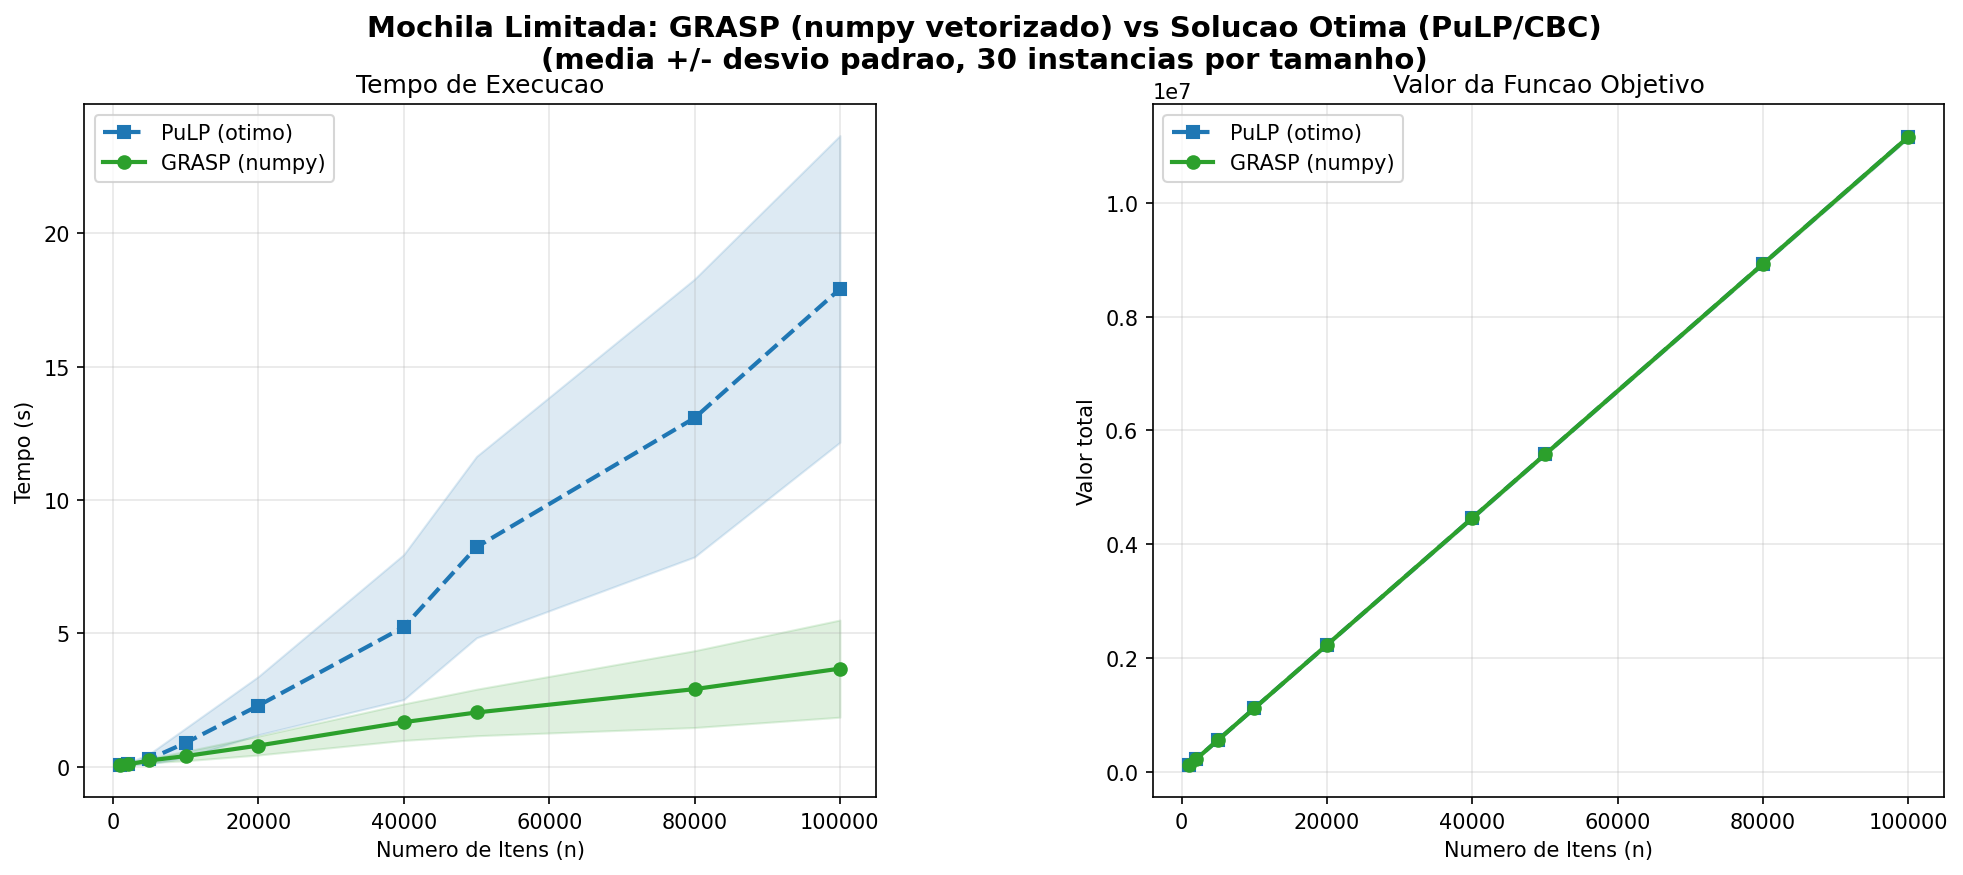
\includegraphics[width=0.92\textwidth]{resultados_grasp.png}
  \end{center}

\end{frame}

% ── Slide 9: Bônus — Comparação de Construtivos ────────────────────────────────
\begin{frame}{Bônus: Comparação entre Mecanismos de Construção}

  \begin{center}
    \textbf{Referência:} Lopes et al.\ (Eds.),
    \emph{Meta-Heurísticas em Pesquisa Operacional}, 2013.
  \end{center}

  \vspace{0.3em}
  \begin{center}
    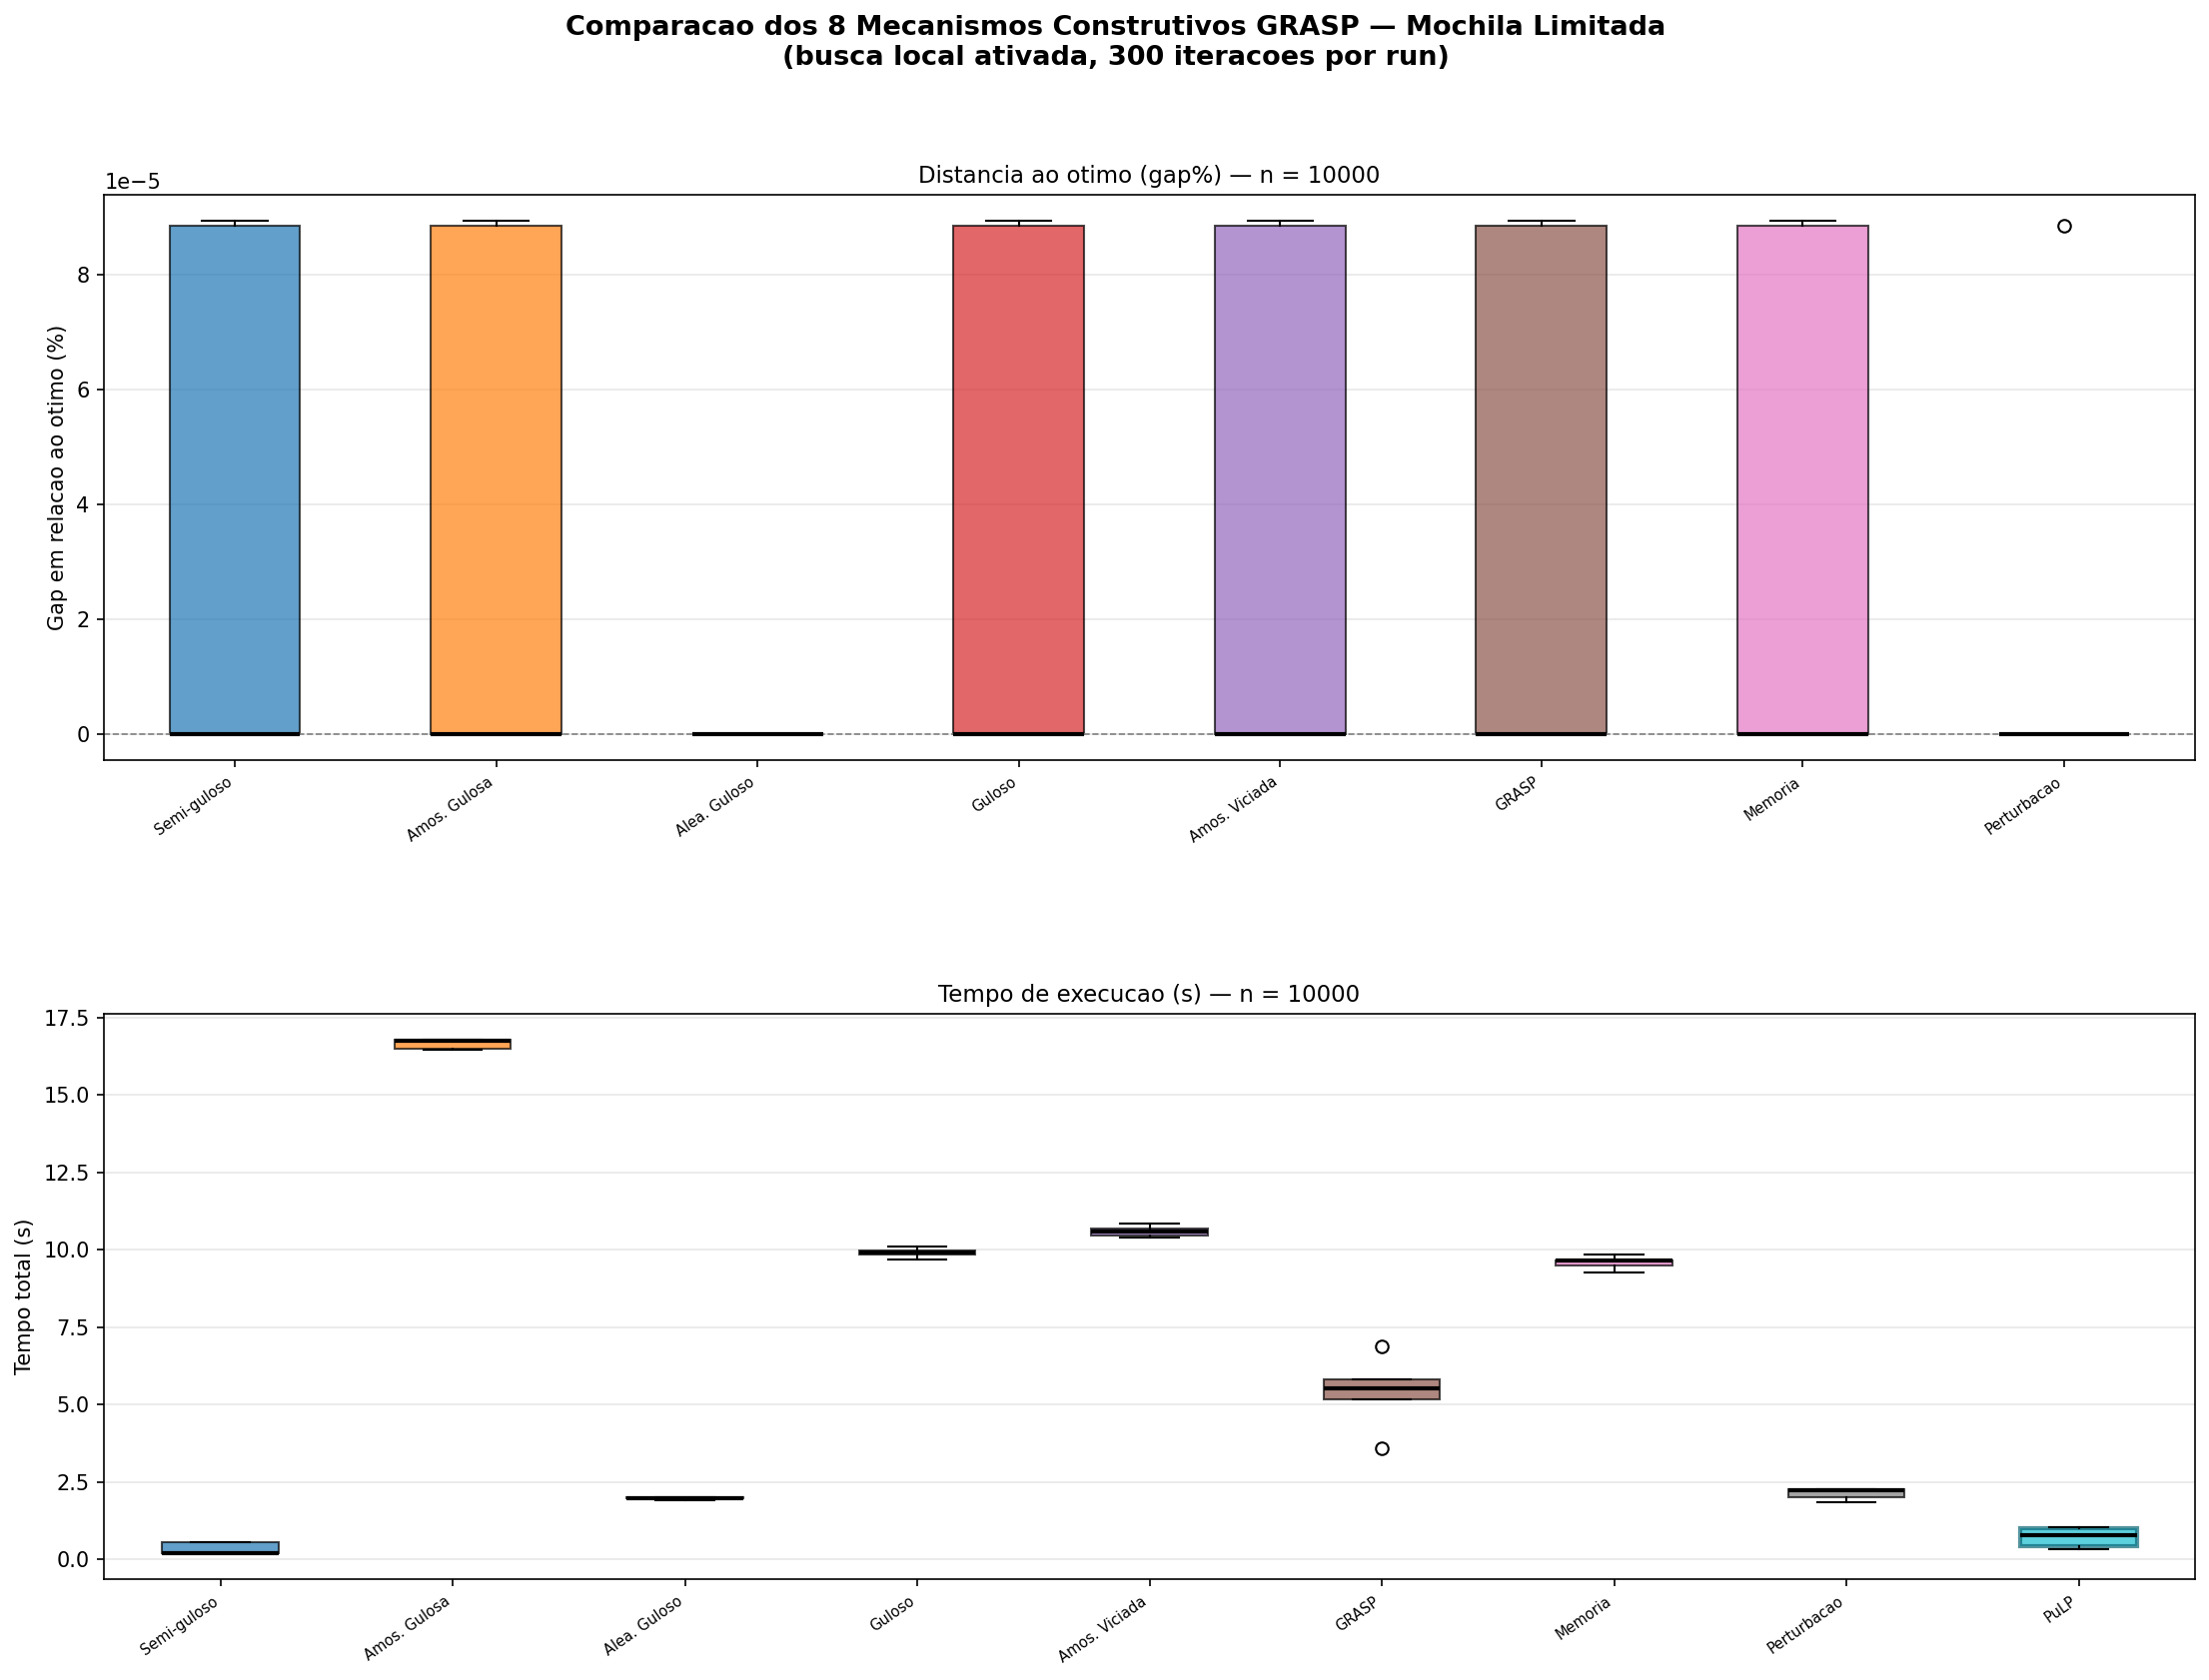
\includegraphics[width=0.88\textwidth]{resultados_construtivos.png}
  \end{center}

\end{frame}

% ── Slide 10: Bibliografia e GitHub ────────────────────────────────────────────
\begin{frame}{Referências e Código}

  \begin{block}{Referências}
    \begin{itemize}
      \item \textbf{Feo, T.\,A. \& Resende, M.\,G.\,C.} (1989).
            A probabilistic heuristic for a computationally difficult set covering problem.
            \emph{Operations Research Letters}, 8:67–71.

      \vspace{0.4em}
      \item \textbf{Lopes, H.\,S. et al.\ (Eds.)} (2013).
            \emph{Meta-Heurísticas em Pesquisa Operacional}.
            Editora Omnipax.
    \end{itemize}
  \end{block}

  \vspace{0.8em}
  \begin{block}{Código-fonte}
    \centering
    \large
    \href{https://github.com/brenopprufrj/mochila-grasp}{github.com/brenopprufrj/mochila-grasp}\\[0.3em]
    \normalsize (Python · NumPy · PuLP · Matplotlib)
  \end{block}

\end{frame}

% ==============================================================================
\end{document}
